\documentclass[french]{article}
 
\usepackage[utf8]{inputenc}
\usepackage[T1]{fontenc}
\usepackage{babel}
\usepackage{advdate}
\usepackage{graphicx} 
\usepackage{amsmath} 
\usepackage{listings}
\usepackage{hyperref}
\usepackage{caption}
\usepackage{subcaption}
\usepackage{listings}

\begin{document}
\begin{titlepage}
\SetDate[29/04/2018]
\newcommand{\HRule}{\rule{\linewidth}{0.5mm}}
\center 
\textsc{\LARGE Université Paris Dauphine}\\[1.5cm] 
\textsc{\Large Data Analytics}\\[0.5cm]
\HRule \\[0.4cm] { \huge \bfseries
Implementation de KMeans avec Spark}\\[0.4cm] \HRule \\[1.5cm]
\begin{minipage}{0.4\textwidth}
	\begin{flushleft} \large
		\emph{Etudiants}
		\\ Elie \textsc{Abi Hanna Daher}
		\\ Bilal \textsc{El Chami}
		\\ Badr \textsc{Erraji}
	\end{flushleft}
\end{minipage}
~
\begin{minipage}{0.4\textwidth}
	\begin{flushright} \large
		\emph{Professeur} 
		\\ M. Benjamin \textsc{Negrevergne}
		\\  \hspace{1cm}
		\\  \hspace{1cm}
	\end{flushright}
\end{minipage}\\[2cm]
{\large \today}\\[2cm]

\includegraphics[width=8cm]{img/dauphine.png}
\vfill
\end{titlepage}
 
\tableofcontents 
\newpage
La méthode K-means est une des méthodes de clustering les plus utilisée lors de l’implémentation d’algorithmes cherchant à regrouper un ensemble de données disparates. Cette méthode repose principalement sur le \textit{unsupervised learning}.
L’objectif étant alors de grouper ces dernières en implémentant l'algorithme KMean avec Spark (python) et en évaluant la performance de notre implémentation basée sur des données que nous générons.


\section{Travail effectué}
\subsection{Implementation}
\subsubsection{Kmeans}
Toutes les fonctions demandées étaient implémentées en respectant le format donné. Ce format nous a énormément aider pour comprendre et développer l’algorithme en suivant le paradigme MapReduce en Spark.\\
Les méthodes de l’algorithme sont les suivantes :
\begin{itemize}
\item \textit{customSplit(…)}
\item \textit{loadData(…)}
\item \textit{initCentroids(…)}
\item \textit{assignToCluster(…)}
\item \textit{calculateDistance(…)}
\item \textit{minDist(…)}
\item \textit{computeCentroids(…)}
\item \textit{reCalculating(…)}
\item \textit{hasConverged(…)}
\item \textit{computeIntraClusterDistance(…)}
\end{itemize}

Les méthodes  \textit{customSplit} et  \textit{loadData} préparent les données passées par l’utilisateur et les formatent en affectant un identifiant pour chaque enregistrement.\\

 \textit{initCentroid} est la fonction critique de l’algorithme qui sert à initialiser les centroïdes. Dans un premier temps, nous avons choisis ces centres aléatoirement parmi les données existantes en utilisant la fonction \textit{takeSample(…)} de la classe RDD. Nous avons implémenté aussi l’algorithme K-means++ qui propose une procédure d’initialisation plus pratique (voire la partie suivante).\\

Ensuite, la méthode \textit{assignToCluster()} prends les données et calcule la distance relative de chaque centroïdes. Puis elle choisit le centroïde ayant la distance minimale, en utilisant les méthodes \textit{calculateDistance()} et \textit{minDist()}, et l’affecte comme cluster de l’enregistrement. Le format utilisé nous a permis de profiter de l’utilisation de la méthode groupByKey de la classe RDD ce qui améliore les performances en passant à l’échelle.\\

Dans la fonction  \textit{computeCentroids()}, nous avons regroupé les résultats d’affectation des clusters, en utilisant autant que possible les fonctions de la classe RDD ( \textit{join()} et  \textit{groupByKey()}). Après avoir grouper les données par cluster, nous avons recalculer les nouvelles valeurs des centroïdes à l’aide de la méthode  \textit{reCalculating()}.

La méthode \textit{computeIntraClusterDistance()} permet de calculer la distance intra-cluster. Cette méthode calcule la somme des moyennes des distances des points aux clusters dont qu'il appartient.\\

Finalement, le programme recalcule à chaque fois les nouvelles valeurs des centroïdes et vérifie si l’algorithme a convergé. La condition de convergence est renvoyé par la méthode  \textit{hasConverged()}.\\

\underline{Observation importante} \\
Une amélioration considérable des performances a été remarqué lors de la modification de l’instruction suivante qui casse le lineage du RDD centroids et crée un nouveau RDD pour l'itération suivante :
\textit{centroids = sc.parallelize(newCentroids.collect())}.
Alors que l’initialisation de centroïdes pouvait se faire de manière aléatoire, ce qui restait fonctionnel. 

\subsubsection{Kmeans++}
L’initialisation de centroïdes pouvait se faire de manière aléatoire, ce qui restait fonctionnel. 

En effet, le fait de générer des centroïdes de manière aléatoire pouvait parfois mener à des situations bloquantes tel que le choix de deux centroids avec exactement les même coordonnées. Par ailleur, le clustering peut donner des résultats différents selon les centroids initiaux choisis qui peuvent parfois être très loin de l’optimum rallongeant les calculs donc avant convergence.

\begin{figure}[h!]
  \centering
  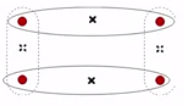
\includegraphics[width=0.4\linewidth]{img/initCentroids.PNG}
  \caption{Initialize centroids}
\end{figure}

Comme nous pouvons le voir sur l’exemple ci-dessus, le clustering peut se faire dans ce cas verticalement ou horizontalement  selon points initiaux.

Nous avons décidé de suivre une autre technique certes quelque peu plus complexe mais qui réduisait le nombre d’itérations considérablement. Nous nous sommes basés sur l’algorithme K-means++ pour implémenter la méthode init centroïdes :

Kmeans ++ a été proposé en 2007 par David Arthur et Sergei Vassilvitskii.\\
Le premier centre du cluster est choisi de manière aléatoire uniforme parmi les points de données. Ensuite, chaque centre de cluster suivant est choisi parmi les points de données restants avec une probabilité proportionnelle à sa distance au carré du centre de cluster existant le plus proche du point.\\
Malheureusement, nous n’avons pas pu implémenter ce dernier en MapReduce à cause de quelques limitations de calcul qui utilisent la librairie numpy. Donc une diminution de performance peut affecter la partie d’initialisation des centroïdes.

\subsubsection{Generateur}
Afin d’évaluer l’algorithme KMeans implémenté, un générateur de données est mis en place. \\

On a mis en place 2 fichiers de python : \textit{generator.py} et \textit{generator-noise.py} \\
Le fichier \textit{generator.py} permet de générer des points et de les sauvegarder dans un fichier. \\
Le deuxième fichier, \textit{generator-noise.py}, permet de générer les points ainsi que des points bruits qui sont générés aléatoirement.\\

Afin de sauvegarder les données dans un fichier externe, on a implémenté 2 façons différentes :
\begin{itemize}
\item 	\textit{saveAsTextFile()} : qui est une méthode déjà présente qui sauvegarde un rdd
\item 	\textit{write-into-csv()} qui est une méthode que nous avons créé qui permet d'écrire directement dans un fichier les valeurs du RDD
\end{itemize}

La méthode que nous avons créé \textit{write-into-csv}, permet de générer un seul fichier mais n'est pas efficiente et ne profite pas des caractéristiques du RDD. C'est pour cela  que la méthode saveAsTextFile est meilleur en terme d'efficacité. Cette dernière crée plusieurs fichiers.

\begin{figure}[h!]
\centering
\begin{subfigure}{.5\textwidth}
  \centering
  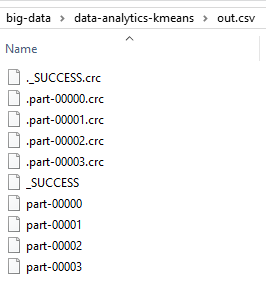
\includegraphics[width=.4\linewidth]{img/save-text-file.png}
  \caption{Méthode \textit{saveAsTextFile}}
  \label{fig:sub1}
\end{subfigure}%
\begin{subfigure}{.5\textwidth}
  \centering
  
\includegraphics[width=.4\linewidth]{img/write-into-csv.png}
  \caption{Méthode \textit{write-into-csv}}
  \label{fig:sub2}
\end{subfigure}
\caption{Fichier output de chaque méthode du générateur de données}
\label{fig:test}
\end{figure}

\newpage
\noindent En exécutant, le \textit{generator.py} avec la commande suivantes :
\begin{lstlisting}[language=bash]
$ spark-submit generator.py out 9 3 2 10
\end{lstlisting}
Les points sont générés, et en affichant les résultats dans le graphique on obtient :
\begin{figure}[h!]
\centering
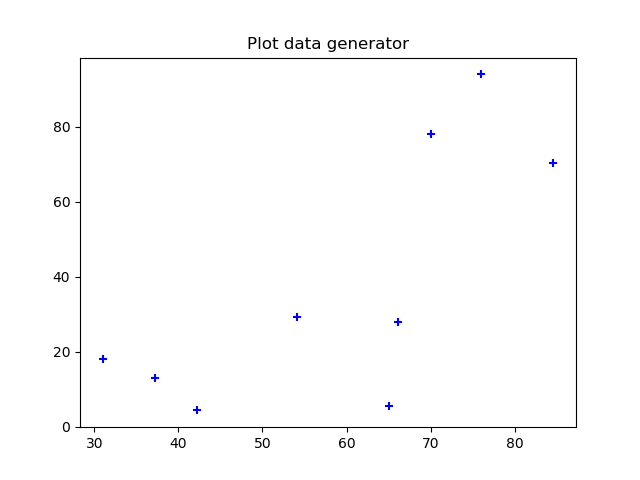
\includegraphics[width=\linewidth]{img/generator-points.png}
\caption{Generateur des points}
\end{figure}

\newpage
\noindent En executant, le \textit{generator-noise.py} avec la commande suivante :
\begin{lstlisting}[language=bash]
$ spark-submit generator_noise.py out 9 3 2 10
\end{lstlisting}
Le nombre de bruits est le double du nombre des points à générer.
Les points sont générés, et en affichant les résultats dans le graphique on obtient :
\begin{figure}[h!]
\centering
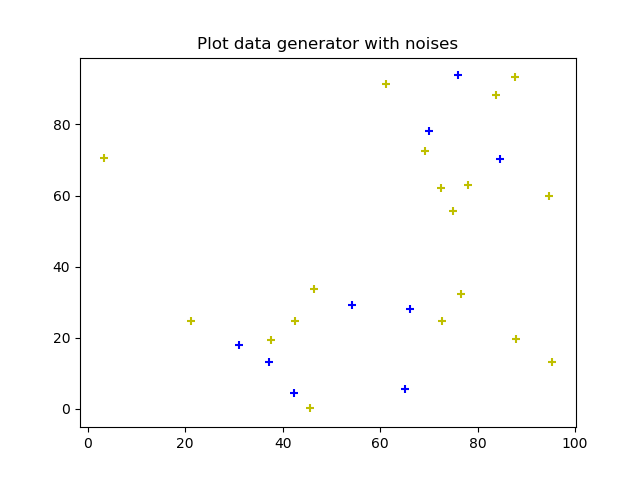
\includegraphics[width=\linewidth]{img/generator-noises.png}
\caption{Générateur des points avec des bruits}
\end{figure}

\newpage
\subsubsection{Plot}
Afin de générer les graphiques, nous avons utilisé la librairie \textit{matplotlib.pyplot}.\\
Pour les fichiers KmeansPlusPlus, Kmeans nous avons créé 2 fichiers pour chacun, 1 sans plot et 1 avec plot.

Pour chaque itération, une image est sauvegardée dans le répertoire afin d'analyser l'évolution du résultat.

Les graphes générés sont de 2 dimensions, ce qui indique que si les points ont plus de 2 coordonnées ca ne seras pas très bien représenté graphiquement.
Afin de voire des exemples d'exécution, veuillez voir la section Simulation.

\subsection{Simulation}
\noindent En exécutant, le \textit{kmeans-plot.py} avec la commande suivantes :
\begin{lstlisting}[language=bash]
$ spark-submit kmeans-plot.py data/iris-small.dat 3 10
\end{lstlisting}

Le graphe suivant représente les résultats de la première itération et en affichant les 2 premiers coordonnées : sepal width et sepal height
\begin{figure}[h!]
\centering
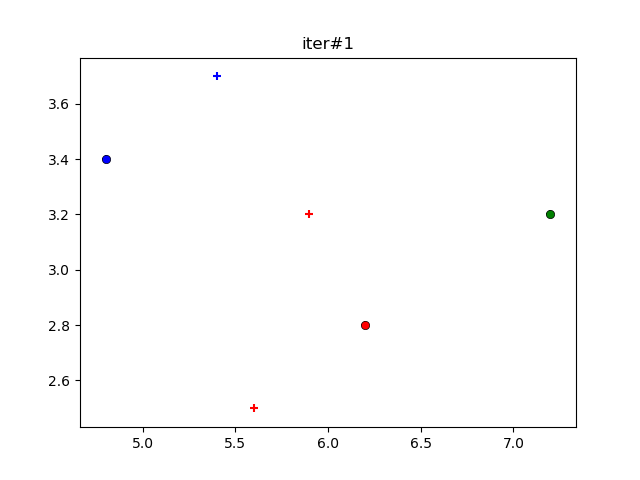
\includegraphics[width=\linewidth]{img/result-kmeans-1.png}
\caption{Iteration 1}
\end{figure}

Pour trouver le resultat final on a eu besoin de 2 iterations avec une distance finale de $0.9711$ d'ou le resultat final est le suivant :
\begin{figure}[h!]
\centering
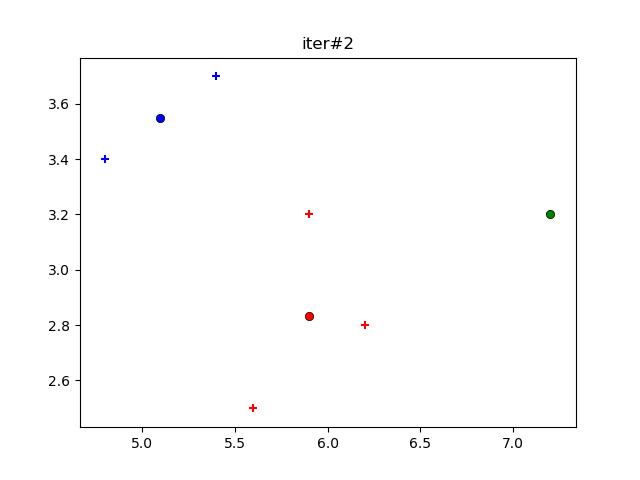
\includegraphics[width=\linewidth]{img/result-kmeans-final.png}
\caption{Iteration finale}
\end{figure}
\newpage 
Et sur la console on obtient le résultat suivant :
\begin{figure}[h!]
\centering
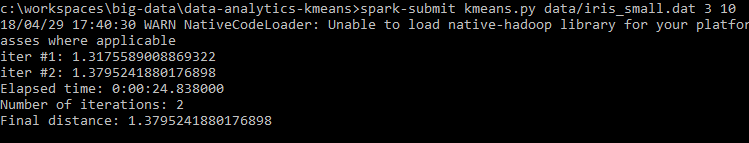
\includegraphics[width=\linewidth]{img/example.png}
\caption{Console}
\end{figure}

\newpage
\subsubsection{Resultat plot - Sepal}
Ci-dessus vous pouvez voire la progression et les résultats de chaque itération sur l'execution de l'algorithm KMeans sur les données iris clustering avec seulement les 2 coordonnées de sepal : sepal width en cm et sepal height en 

\begin{figure}[h!]
\centering
\begin{subfigure}{.5\textwidth}
  \centering
  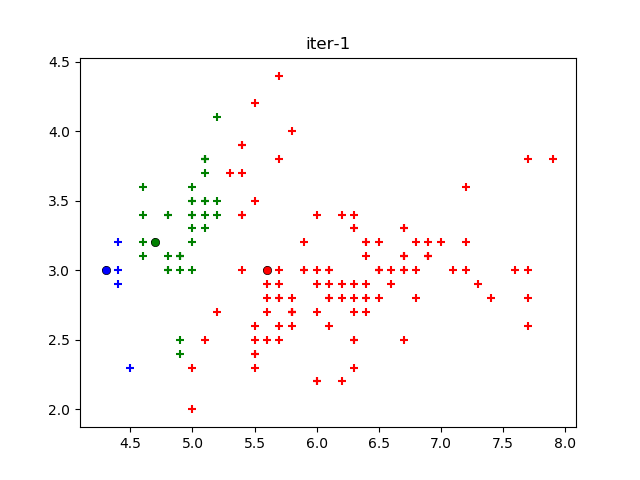
\includegraphics[width=\linewidth]{img/iter-1.png}
  \caption{Iteration 1}
\end{subfigure}%
\begin{subfigure}{.5\textwidth}
  \centering
  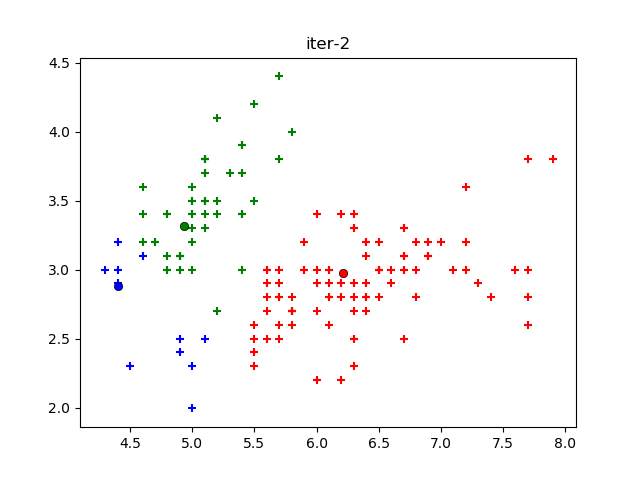
\includegraphics[width=\linewidth]{img/iter-2.png}
  \caption{Iteration 2}
\end{subfigure}%
\end{figure}

\begin{figure}[h!]
\centering
\begin{subfigure}{.5\textwidth}
  \centering
  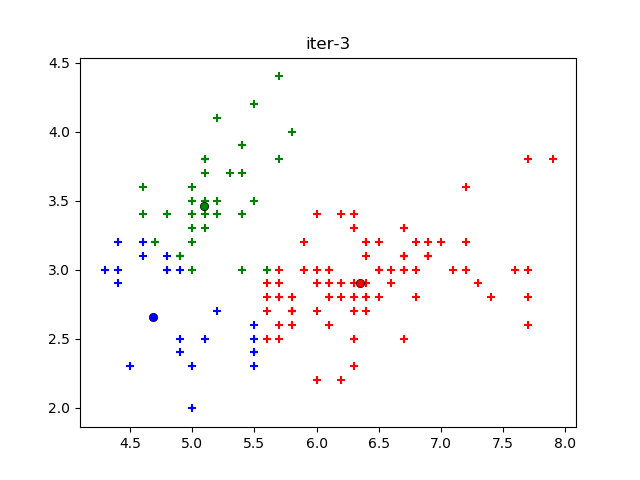
\includegraphics[width=\linewidth]{img/iter-3.png}
  \caption{Iteration 3}
\end{subfigure}%
\begin{subfigure}{.5\textwidth}
  \centering
  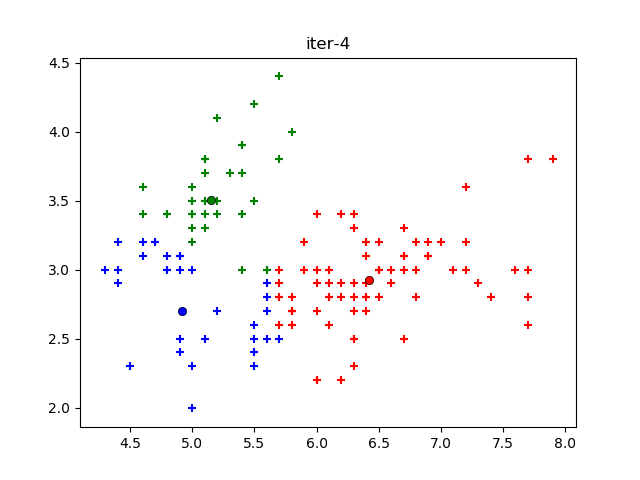
\includegraphics[width=\linewidth]{img/iter-4.png}
  \caption{Iteration 4}
\end{subfigure}%
\end{figure}

\newpage
\begin{figure}[h!]
\centering
\begin{subfigure}{.5\textwidth}
  \centering
  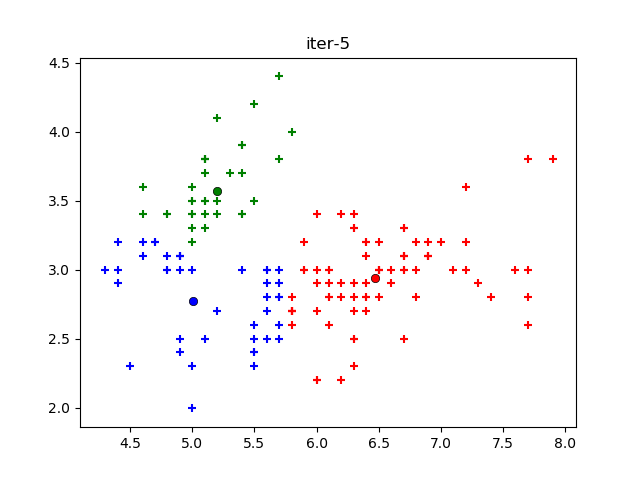
\includegraphics[width=\linewidth]{img/iter-5.png}
  \caption{Iteration 5}
\end{subfigure}%
\begin{subfigure}{.5\textwidth}
  \centering
  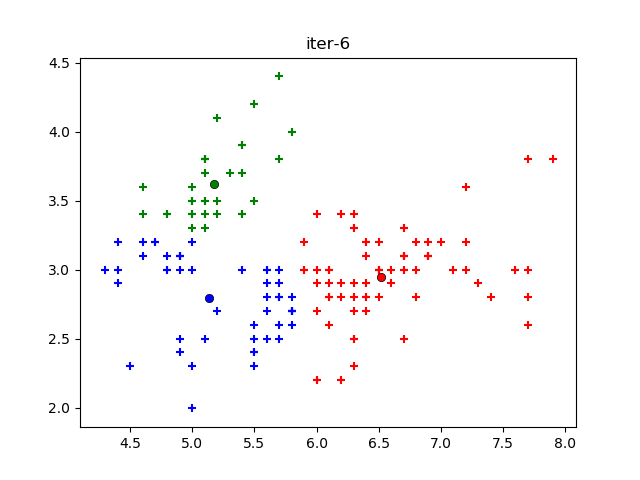
\includegraphics[width=\linewidth]{img/iter-6.png}
  \caption{Iteration 6}
\end{subfigure}%
\end{figure}

\begin{figure}[h!]
\centering
\begin{subfigure}{.5\textwidth}
  \centering
  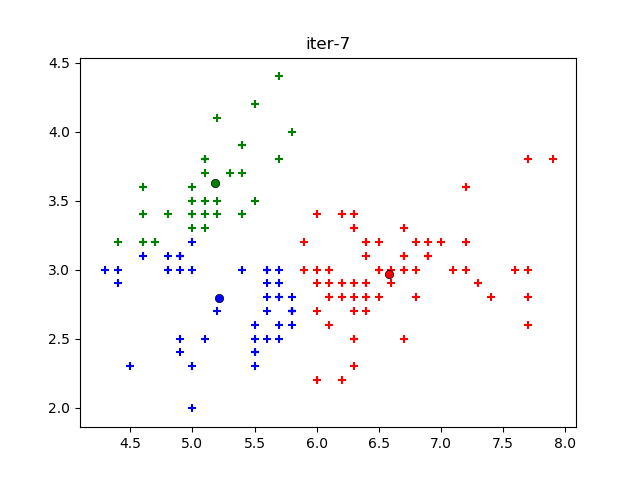
\includegraphics[width=\linewidth]{img/iter-7.png}
  \caption{Iteration 7}
\end{subfigure}%
\begin{subfigure}{.5\textwidth}
  \centering
  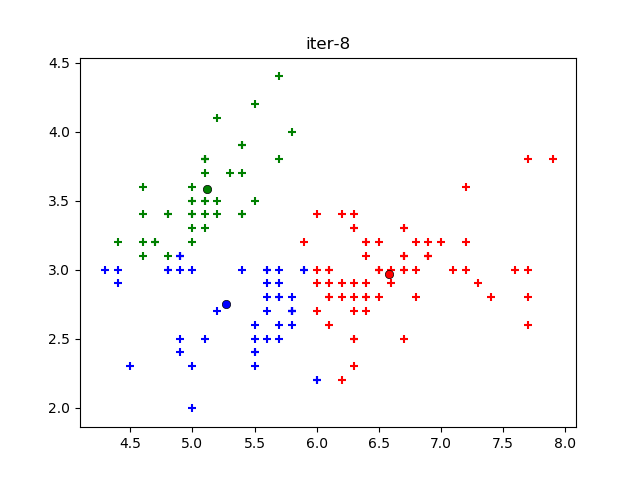
\includegraphics[width=\linewidth]{img/iter-8.png}
  \caption{Iteration 8}
\end{subfigure}%
\end{figure}


\newpage

\begin{figure}[h!]
\centering
\begin{subfigure}{.5\textwidth}
  \centering
  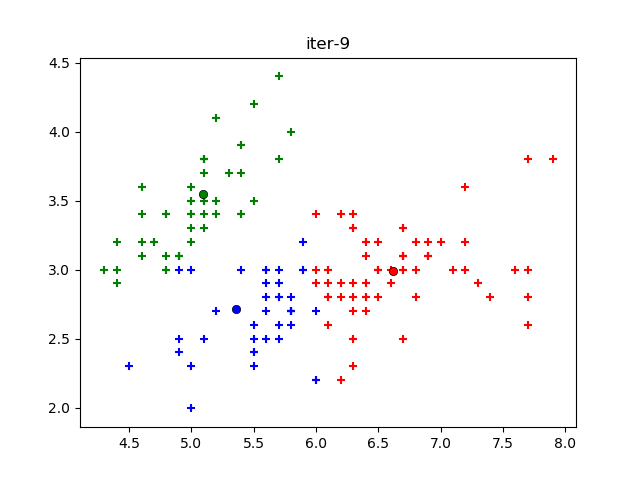
\includegraphics[width=\linewidth]{img/iter-9.png}
  \caption{Iteration 9}
\end{subfigure}%
\begin{subfigure}{.5\textwidth}
  \centering
  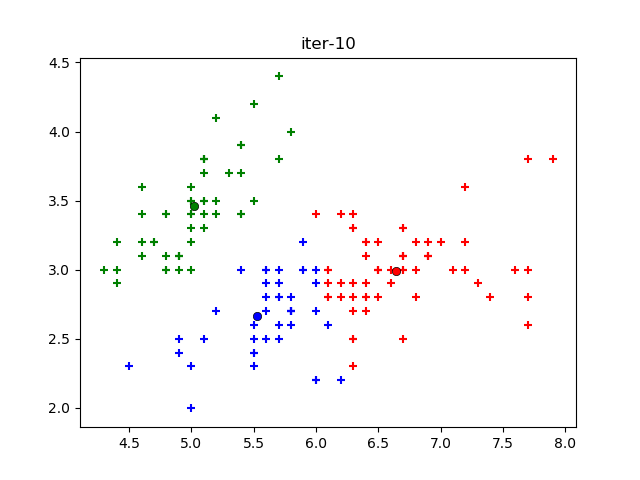
\includegraphics[width=\linewidth]{img/iter-10.png}
  \caption{Iteration 10}
\end{subfigure}%
\end{figure}

\begin{figure}[h!]
\centering
\begin{subfigure}{.5\textwidth}
  \centering
  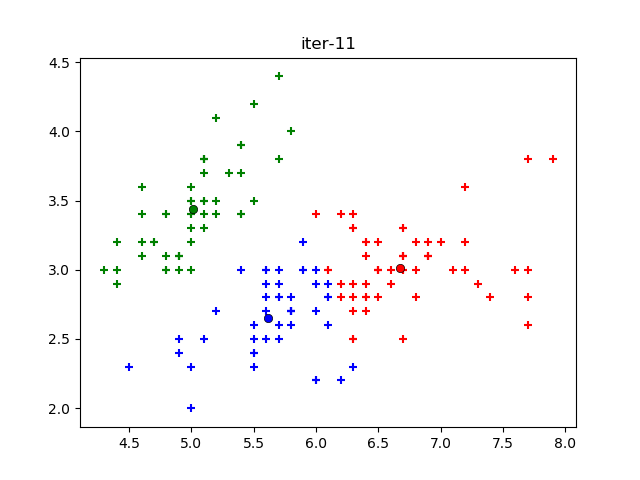
\includegraphics[width=\linewidth]{img/iter-11.png}
  \caption{Iteration 11}
\end{subfigure}%
\begin{subfigure}{.5\textwidth}
  \centering
  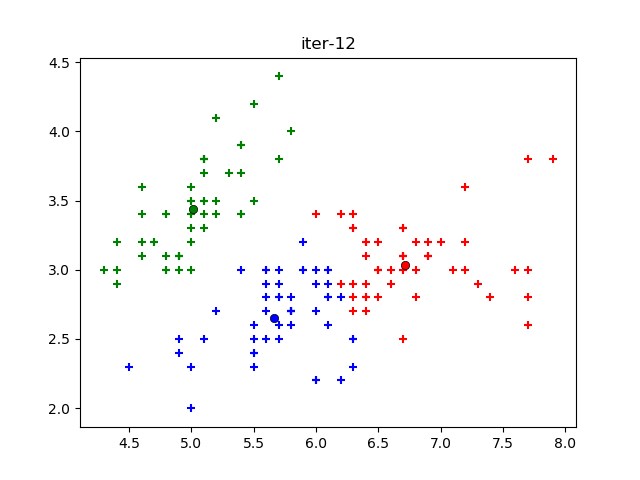
\includegraphics[width=\linewidth]{img/iter-12.png}
  \caption{Iteration 12}
\end{subfigure}%
\end{figure}


\newpage

\begin{figure}[h!]
\centering
\begin{subfigure}{.5\textwidth}
  \centering
  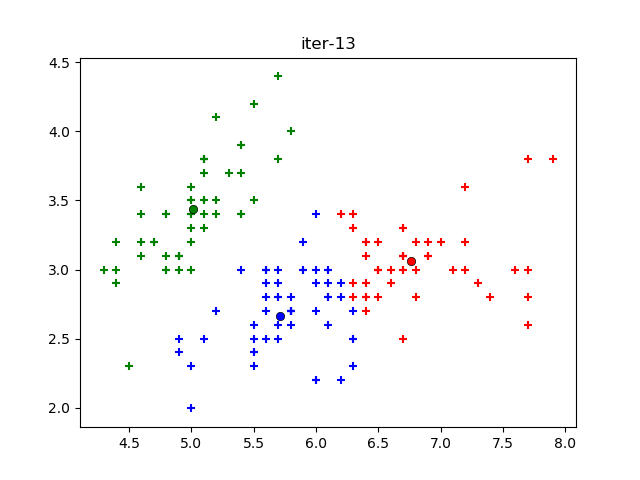
\includegraphics[width=\linewidth]{img/iter-13.png}
  \caption{Iteration 13}
\end{subfigure}%
\begin{subfigure}{.5\textwidth}
  \centering
  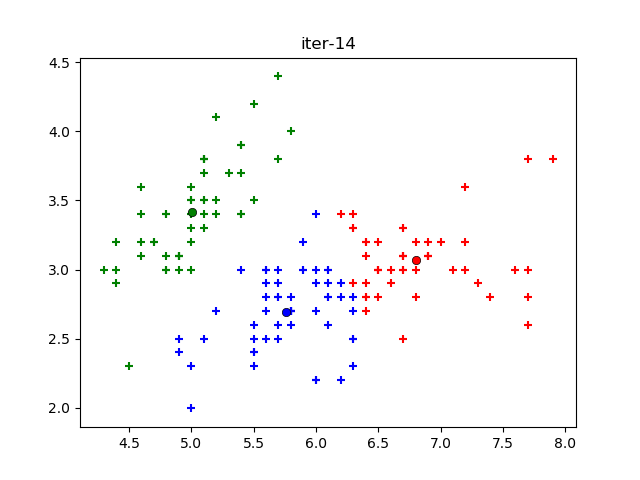
\includegraphics[width=\linewidth]{img/iter-14.png}
  \caption{Iteration 14}
\end{subfigure}%
\end{figure}
\begin{figure}[h!]
\centering
\begin{subfigure}{.5\textwidth}
  \centering
  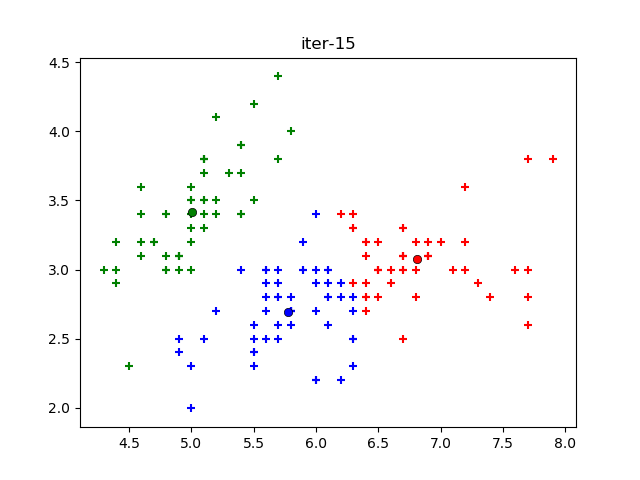
\includegraphics[width=\linewidth]{img/iter-15.png}
  \caption{Iteration 15}
\end{subfigure}%
\end{figure}

\begin{itemize}
\item Temps d'exécution : 4 min 20 sec
\item Iitérations: 15
\item Distance: 1.259
\end{itemize}


\newpage
\subsubsection{Resultat plot - Petal}
Ci-dessus vous pouvez voire la progression et les résultats de chaque itération sur l'execution de l'algorithm KMeans sur les données iris clustering avec seulement les 2 coordonnées  de sepal : petal width en cm et petal height en 

\begin{figure}[h!]
\centering
\begin{subfigure}{.5\textwidth}
  \centering
  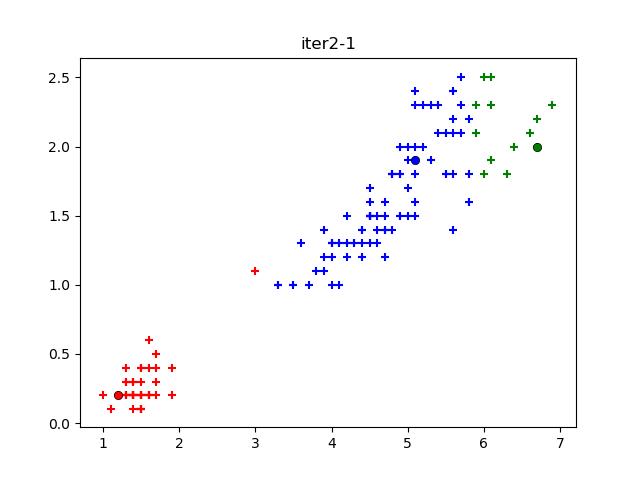
\includegraphics[width=\linewidth]{img/iter2-1.png}
  \caption{Iteration 1}
\end{subfigure}%
\begin{subfigure}{.5\textwidth}
  \centering
  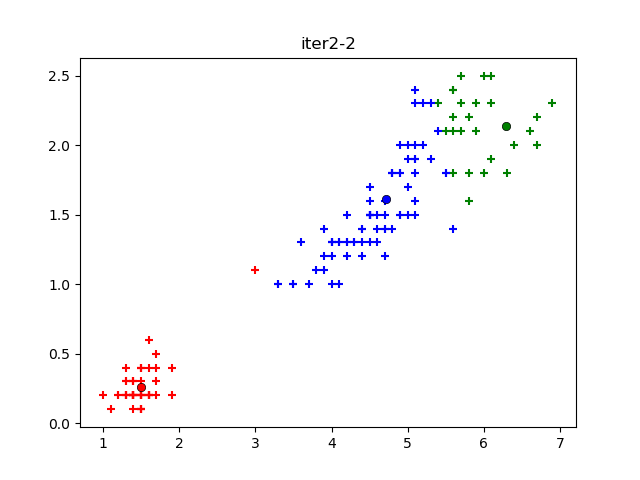
\includegraphics[width=\linewidth]{img/iter2-2.png}
  \caption{Iteration 2}
\end{subfigure}%
\end{figure}

\begin{figure}[h!]
\centering
\begin{subfigure}{.5\textwidth}
  \centering
  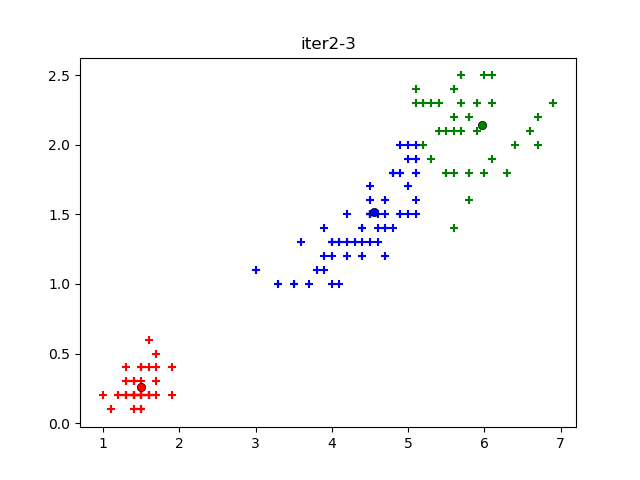
\includegraphics[width=\linewidth]{img/iter2-3.png}
  \caption{Iteration 3}
\end{subfigure}%
\begin{subfigure}{.5\textwidth}
  \centering
  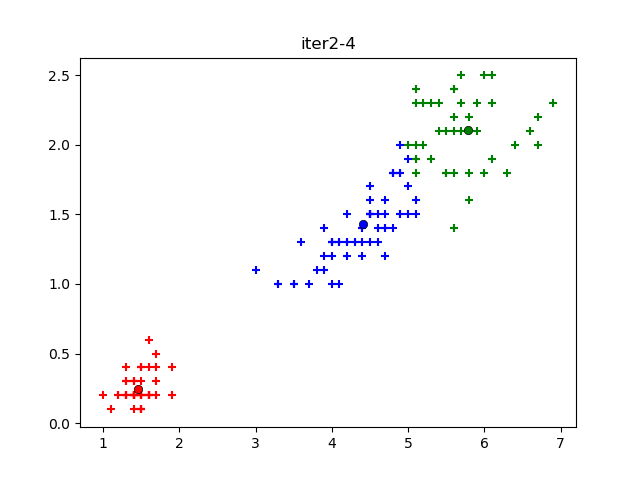
\includegraphics[width=\linewidth]{img/iter2-4.png}
  \caption{Iteration 4}
\end{subfigure}%
\end{figure}

\newpage
\begin{figure}[h!]
\centering
\begin{subfigure}{.5\textwidth}
  \centering
  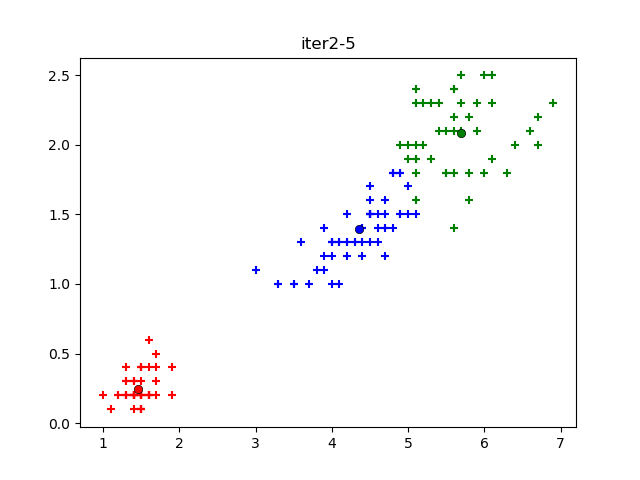
\includegraphics[width=\linewidth]{img/iter2-5.png}
  \caption{Iteration 5}
\end{subfigure}%
\begin{subfigure}{.5\textwidth}
  \centering
  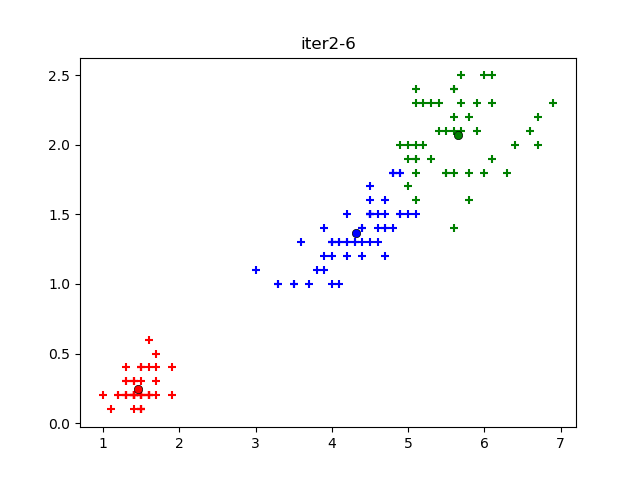
\includegraphics[width=\linewidth]{img/iter2-6.png}
  \caption{Iteration 6}
\end{subfigure}%
\end{figure}

\begin{figure}[h!]
\centering
\begin{subfigure}{.5\textwidth}
  \centering
  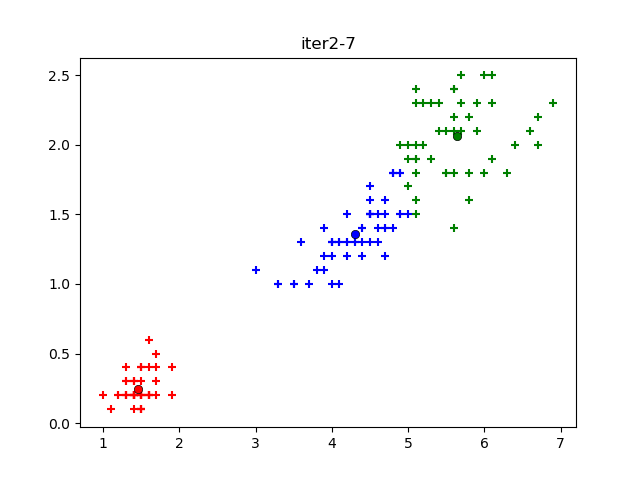
\includegraphics[width=\linewidth]{img/iter2-7.png}
  \caption{Iteration 7}
\end{subfigure}%
\begin{subfigure}{.5\textwidth}
  \centering
  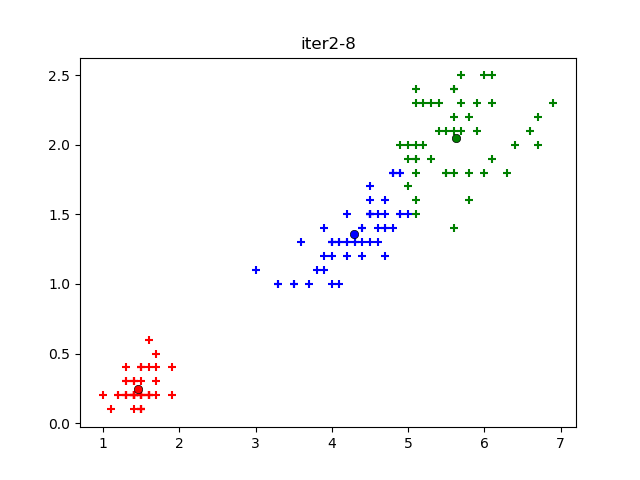
\includegraphics[width=\linewidth]{img/iter2-8.png}
  \caption{Iteration 8}
\end{subfigure}%
\end{figure}


\begin{itemize}
\item Temps d'exécution : 2 min 20 sec
\item Iitérations: 8
\item Distance: 1.1143
\end{itemize}

\newpage
\section{Analyse}
\subsection{Distance intra-cluster}
En exécutant le programme, nous avons bien remarqué que la distance intra-cluster diminue progressivement jusqu'à atteindre un minimum durant la derniere iteration. On aperçoit parfois une légère augmentation suivi d’une diminution notable.\\

\subsection{Convergence}
L’algorithme s'arrête dès que les centroïdes gardent leurs valeurs durant deux itérations consécutives.

K-means avec une initialisation aléatoire des centres converge en 7 iterations, tandis que k-means++ réussi à converger en 6 iterations.

\subsection{Tableau de performance}

    \begin{table}[!hbt]
        \begin{center}
        \caption{ 100 executions }
        \label{tab:simParameters}
        \begin{tabular}{|c|c|c|c|}
            \hline
           Algorithme & Temps d'exécution & Iterations  & Distance finale \\
            \hline
           KMeans - implémenté & $10.25$ s & $6.75$ & $2.41$ \\
            \hline
           KMeans ++- implémenté & $9.5$ s & $6.35$ & $2.41$  \\
            \hline      
        \end{tabular}
        \end{center}
    \end{table}

\section{Application}
Afin de tester sur plus de données, nous avons créer notre propre données. Nous avons collecté la taille ainsi que le poid de 92 jours de Basket de la NBA et leur position represente leurs cluster. (voire dans le repertoire data : nba.csv).

Donc notre but c'est de voir si c'est 2 coordonnées : taille (m) et poid (kg) on une forte relation avec la position des joueurs.

Donc en exécutant l'algorithme on obtient les resultat suivantes : 
\begin{itemize}
\item Temps d'exécution : 48 sec
\item Iitérations: 2
\item Distance: 14.9
\end{itemize}

\begin{figure}[h!]
\centering
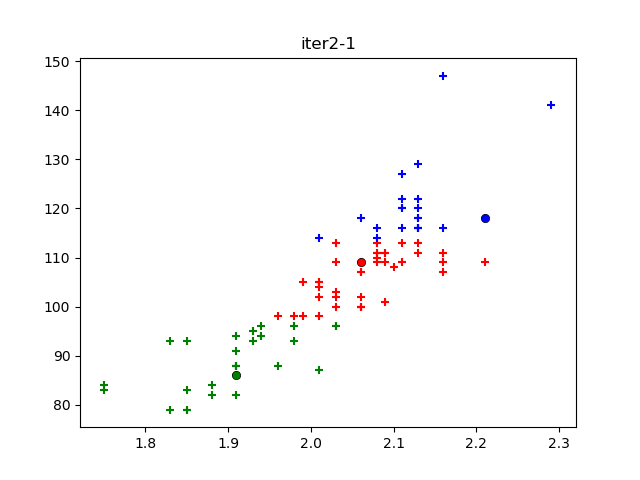
\includegraphics[width=\linewidth]{img/nba-iter1.png}
\caption{Iteration 1}
\end{figure}
\newpage

\begin{figure}[h!]
\centering
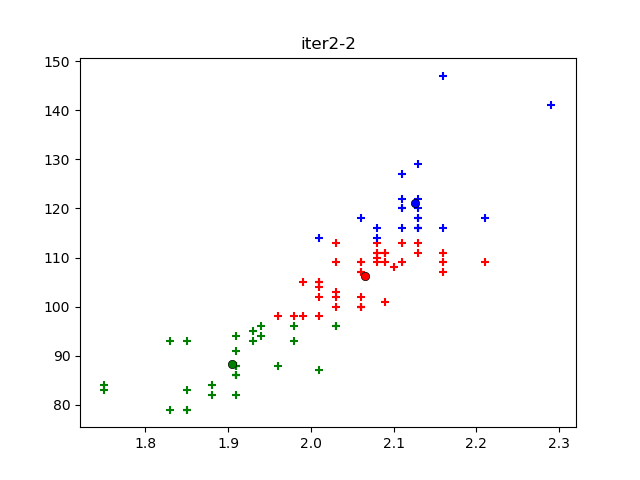
\includegraphics[width=\linewidth]{img/nba-iter2.png}
\caption{Iteration 2}
\end{figure}

On remarque ici que les données sont assez répartis:
\begin{itemize}
\item les joueurs qui ont un petit poid et une petit taille sont regroupé (Guards)
\item les joueurs qui ont un moyen poid et une moyenne taille sont regroupé (Forwards)
\item les joueurs qui ont un grand poin et une grande taille sont regroupé (Center)
\end{itemize} 

\newpage

\begin{thebibliography}{5}
    \bibitem{MonteCarloKakuro} 
    KMeans ++ in python   [Online]. \\ Disponible:  \url{https://datasciencelab.wordpress.com/2014/01/15/improved-seeding-for-clustering-with-k-means/}
   \bibitem{WikiKakuro} 
   Donnée de test sur Archive ICS UCI. [Online]. \\ Disponible:  \url{ https://archive.ics.uci.edu/ml/machine-learning-databases/soybean/soybean-small.data}
   \bibitem{bla} 
   Initialization of k means clustering [Online]. \\ Disponible:  \url{https://www.coursera.org/learn/cluster-analysis/lecture/bPyBl/3-3-initialization-of-k-means-clustering}
   \bibitem{test1} 
   K-means clustering: how it works [Online]. \\ Disponible:  \url{ https://www.youtube.com/watch?v=_aWzGGNrcic}
   \bibitem{test2} 
   Scalable K Means++ . [Online]. \\ Disponible:  \url{ https://www.youtube.com/watch?v=KHu8uNy4pV8&t=924s}



\end{thebibliography}
\end{document}